% 请确保文件编码为utf-8,使用XeLaTex进行编译,或者通过overleaf进行编译

\documentclass[answers]{exam}  % 使用此行带有作答模块
% \documentclass{exam} % 使用此行只显示题目

\usepackage{xeCJK}
\usepackage{zhnumber}
\usepackage{graphicx}
\usepackage{hyperref}
\usepackage{amsmath}
\usepackage{booktabs}
\usepackage{enumerate}
\usepackage{amssymb}

\pagestyle{headandfoot}
\firstpageheadrule
\firstpageheader{南京大学}{高级机器学习}{习题集三}
\runningheader{南京大学}
{高级机器学习}
{习题集三}
\runningheadrule
\firstpagefooter{}{第\thepage\ 页(共\numpages 页)}{}
\runningfooter{}{第\thepage\ 页(共\numpages 页)}{}

% no box for solutions
% \unframedsolutions

\setlength\linefillheight{.5in}

% \renewcommand{\solutiontitle}{\noindent\textbf{答:}}
\renewcommand{\solutiontitle}{\noindent\textbf{解:}\par\noindent}

\renewcommand{\thequestion}{\zhnum{question}}
\renewcommand{\questionlabel}{\thequestion .}
\renewcommand{\thepartno}{\arabic{partno}}
\renewcommand{\partlabel}{\thepartno .}


\begin{document}
\Large

\begin{questions}
\question [30] \textbf{计算学习理论}

	本题探讨计算学习理论章节中VC 维的性质。
	
	\begin{parts}
		\part [10] 请在样本空间~$\mathcal{X} = [0,1]$~上构造一个有限假设空间~$\mathcal{H}$~使得~$\mbox{VC}(\mathcal{H}) = \left \lfloor \log_2(\left| \mathcal{H} \right| ) \right \rfloor $.
		
		\part [10] 定义轴平行四边形概念类~$\mathcal H = \{h_{(a_1, a_2, b_1, b_2)}(x, y): a_1\le a_2 \land b_1\le b_2\}$, 其中
		\[ h_{(a_1, a_2, b_1, b_2)}(x, y) = \begin{cases}
			1&\quad \text{ if } a_1\le x\le a_2 \land b_1\le y \le b_2 \\
			0 & \quad \text{otherwise}
		\end{cases}
		\]
		请证明~$\mathcal H$~的~VC~维为~4.
		
		\part [10] 请证明最近邻分类器的假设空间的~VC~维可以为无穷大.
		
	\end{parts}

	\begin{solution}
		\begin{parts}
			\part 
			\part 
			\part 
		\end{parts}
	\end{solution}


\question [40] \textbf{编程题:特征工程和规则学习}

	\begin{figure}
		\centering
		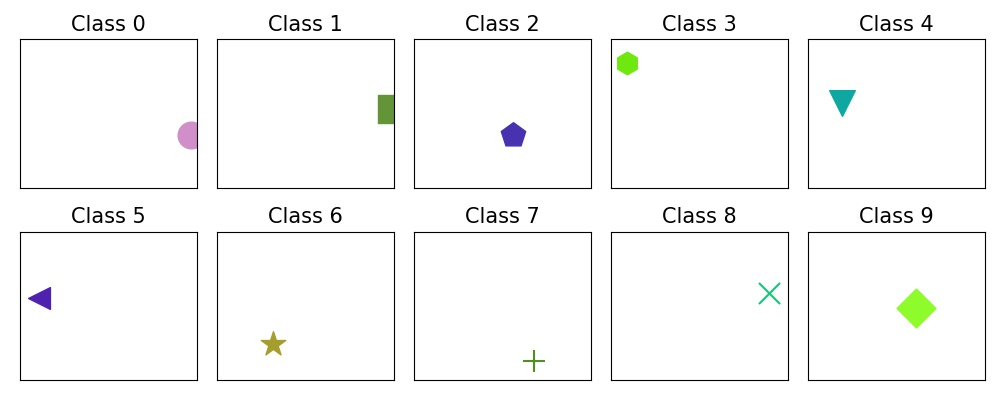
\includegraphics[width=0.7\linewidth]{problem2-code/demos/demo-0.jpg}
		\caption{图案分类问题示例图} \label{fig:q2-demo}
	\end{figure}

	本题涉及一个简单的图像识别问题,主要是对示例图~\ref{fig:q2-demo}中的10种图案进行识别,图案有不同大小、不同颜色,并且处在图像中不同位置,即不一定在中心位置,可能出现部分观测(某部分可能缺失,例如图中的Class 0)。分类依据主要是其形状,例如五角星、三角形、加号、正方形等等。本题代码文件夹在``problem2-code"目录下。\textbf{请在作答中贴出核心代码文件和结果,以方便批改。}
	
	\begin{parts}
		\part [10] 根据``generate\_samples.py"生成训练测试图片,其中n\_samples控制了训练测试样本中每个类别的数目,示例文件设置为200,那么训练测试集各有2000个样本。生成好图像之后,``load\_data.py"提供了读取图像数据的示例代码,``train\_p0.py"提供了使用对数几率回归(Logistic Regression)、决策树(Decision Tree)、随机森林(Random Forest)进行分类的示例代码。该代码还提供了可做PCA降维的选项。该代码没有提取任何特征,只是对图像缩放为32 * 32大小的彩色图像,然后使用所有像素点组成的向量进行分类。尝试运行该代码,将结果记录下来。此外,鼓励使用更多的分类器、更多的超参数设置、更多的数据进行训练,对比一下这些设置是否可以提升性能?例如:增加训练数据数量是否会提升性能?
		\part [10] 考虑到图像分类只和其形状有关,和其大小、位置、颜色无关,所以尝试将图像变为灰度图、定位目标的中心位置并进行裁剪等操作,然后再进行同样的训练。试着比较这种数据预处理带来的性能提升。提示:高阶的数据预处理还可以将灰度图变为轮廓图或者提取边缘信息等。
		\part [10] 上述虽然去除了一些和分类任务无关的信息(例如:颜色),但是其使用的特征依然是像素点信息。尝试手动提取高质量的特征,例如:图案中直线的数量、直线角度、直线之间的位置关系、图案的面积等等。试着以尽量少的特征获得更好的分类性能。提取的特征越少,性能越好,分数越高。
		\part [10] 在上一问中,使用决策树进行分类。本质上决策树就是一系列规则,尝试将决策树训练得到的模型使用文本或者图形将这一系列规则描述出来,观察是否符合预期(例如: 有一条水平和一条垂直线的是加号),从而更加深入地了解该模型。
	\end{parts}
	
	\begin{solution}
		\begin{parts}
			\part 
			\part 
			\part 
			\part 
		\end{parts}
	\end{solution}


\question [30] \textbf{编程题:强化学习}
	\begin{figure}
		\centering
		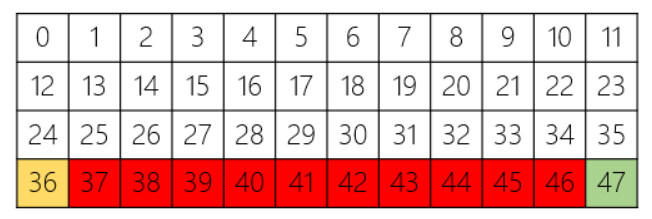
\includegraphics[width=0.7\linewidth]{problem3-code/env.PNG}
		\caption{悬崖行走问题示例图} \label{fig:q3-env}
	\end{figure}

	悬崖行走问题定义如下: 问题环境为如图~\ref{fig:q3-env}所示的4 * 12方格,智能体初始在36号位置,每次可上下左右移动一格,遇到墙则原地不动。每次移动获得-1奖励。37-46号位置为悬崖,若移动至悬崖,获得-100奖励并回到原点36号位置。47号位置为终点,运行至此为结束。总奖励为各步奖励之和。问题参数:$\epsilon=0.1,\alpha=0.5,\gamma=1$。\\
	请在悬崖行走问题中分别实现Sarsa算法与Q-learning算法,并分别输出运用两种算法训练得到的路径。本题代码文件夹在``problem3-code"目录下。问题环境可自己写,也可直接利用``cliff\_walking.py"文件中的Env类。\textbf{请在作答中贴出核心代码文件和结果,以方便批改。}
	
	\begin{solution}
		
	\end{solution}
	
\end{questions}


\end{document}